\par Sprawne działanie przedsiębiorstwa zależy od możliwości przetwarzania informacji, w szczególności w firmach o profilu handlowym. Informacją będzie komunikacja między klientami i przedsiębiorstwem oraz producentami i przedsiębiorstwem. Informacje te możemy podzielić na powstałe w procesach zamówienia, produkcji i dostawy. Przepływem informacji będzie też komunikacja między pracownikami, czy przygotowanie katalogu produktów. Do przepływu informacji możemy również zaliczyć komunikacje z instytucjami administracyjnymi. Celem zapewnienia nieprzerwanego przepływu informacji konieczne jest utworzenie systemu pozwalającego realizować powyższe założenia. Na tej podstawie, przedsiębiorstwo można zobrazować jako centrum wymiany informacji. Wymiana ta zachodzi między grupami pracowników, producentów, klientów i firmami transportowymi.
		
		\begin{figure}[H]
			\centering
			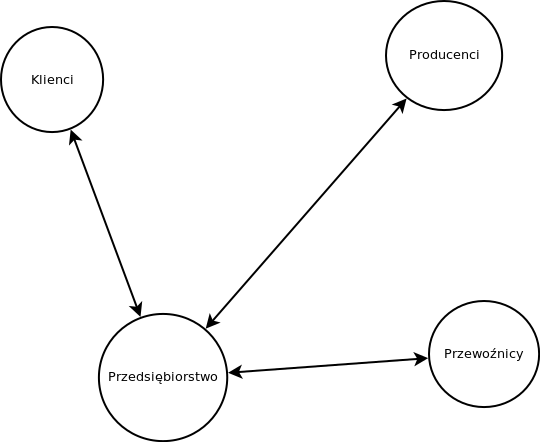
\includegraphics[scale=0.45]{groups}
			\caption{Przepływ informacji między grupami ludzi}
			\label{groups}
		\end{figure} 
